
\documentclass[a4paper,11pt]{article}
\usepackage{geometry}
\geometry{margin=2cm}
\usepackage{booktabs}
\usepackage{graphicx}
\usepackage{amsmath}
\usepackage{siunitx}
\usepackage{caption}
\usepackage{times}
\usepackage[utf8]{inputenc}
\usepackage{tocloft}

\title{Spectral Simulation Report}
\author{Automated Analysis}
\date{\today}

\begin{document}

\maketitle
\tableofcontents
\clearpage

\section{Introduction}
This report presents the results of spectral simulations derived from HDF5 dataset analysis. Each sample includes a spectral plot and a detailed table summarizing the initial composition and actual labeled positions of elements, along with simulation parameters such as temperature and electron density.


\section{Sample: 16197}
\subsection{Simulation Parameters}
\begin{table}[h!]
    \centering
    \begin{tabular}{ll}
        \toprule
        \textbf{Parameter} & \textbf{Value} \\
        \midrule
        Temperature ($T$) & 9040 \,\si{K} \\
        Electron Density ($n_e$) & 7.92e+15 \,\si{cm^-3} \\
        \bottomrule
    \end{tabular}
    \caption{Simulation parameters for sample 16197.}
    \label{tab:params_16197}
\end{table}

\subsection{Composition Analysis}
\begin{table}[h!]
    \centering
    \begin{tabular}{lcc}
        \toprule
        \textbf{Element} & \textbf{Initial Composition (\%)} & \textbf{Actual Labeled Position (\%)} \\
        \midrule
        Al & 10.87 & 10.74 \\
        Ar & 0.00 & 0.00 \\
        C & 0.00 & 0.00 \\
        Ca & 6.83 & 3.66 \\
        Cl & 7.15 & 0.66 \\
        Co & 6.13 & 34.28 \\
        Cr & 10.34 & 9.69 \\
        Fe & 0.00 & 0.00 \\
        Mg & 10.49 & 8.47 \\
        Mn & 11.31 & 17.24 \\
        N & 5.84 & 9.69 \\
        Na & 3.75 & 7.86 \\
        Ni & 3.52 & 11.67 \\
        O & 7.31 & 4.05 \\
        S & 7.85 & 5.05 \\
        Si & 8.63 & 5.44 \\
        Ti & 0.00 & 0.00 \\
        background & N/A & 28.64 \\

        \midrule
        \textbf{Total (\%)} & & 157.15 \\
        \bottomrule
    \end{tabular}
    \caption{Composition analysis for sample 16197.}
    \label{tab:comp_16197}
\end{table}

\subsection{Spectral Plot}
\begin{figure}[h!]
    \centering
    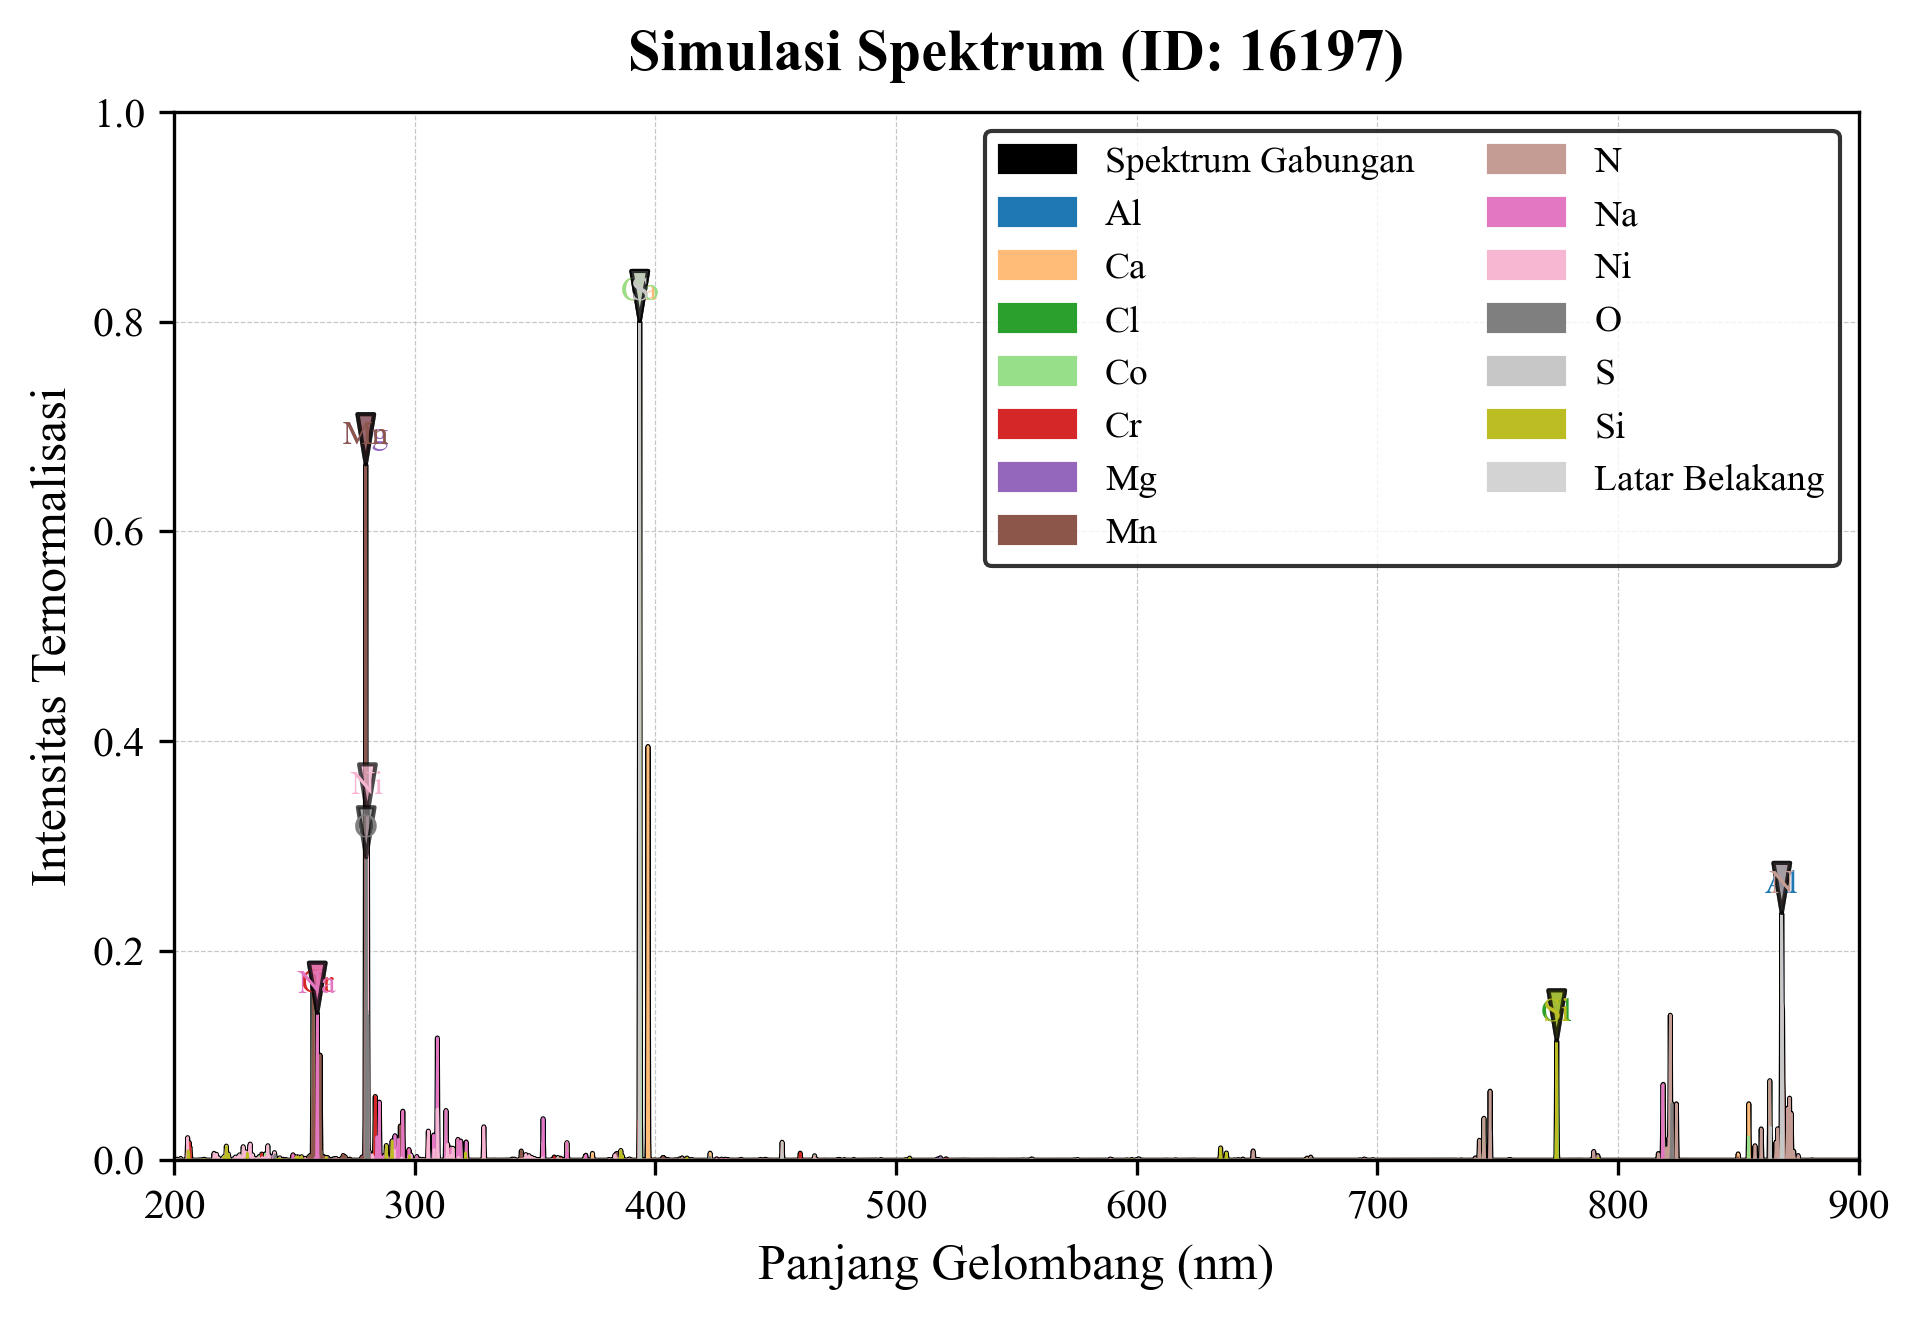
\includegraphics[width=0.9\textwidth]{spectrum_16197.png}
    \caption{Spectral simulation plot for sample 16197.}
    \label{fig:spectrum_16197}
\end{figure}

\clearpage

\section{Sample: 5639}
\subsection{Simulation Parameters}
\begin{table}[h!]
    \centering
    \begin{tabular}{ll}
        \toprule
        \textbf{Parameter} & \textbf{Value} \\
        \midrule
        Temperature ($T$) & 10556 \,\si{K} \\
        Electron Density ($n_e$) & 3.13e+15 \,\si{cm^-3} \\
        \bottomrule
    \end{tabular}
    \caption{Simulation parameters for sample 5639.}
    \label{tab:params_5639}
\end{table}

\subsection{Composition Analysis}
\begin{table}[h!]
    \centering
    \begin{tabular}{lcc}
        \toprule
        \textbf{Element} & \textbf{Initial Composition (\%)} & \textbf{Actual Labeled Position (\%)} \\
        \midrule
        Al & 0.00 & 0.00 \\
        Ar & 0.00 & 0.00 \\
        C & 0.00 & 0.00 \\
        Ca & 5.56 & 3.66 \\
        Cl & 14.21 & 0.85 \\
        Co & 11.98 & 34.28 \\
        Cr & 8.58 & 9.69 \\
        Fe & 0.00 & 0.00 \\
        Mg & 4.15 & 8.57 \\
        Mn & 3.40 & 17.24 \\
        N & 2.14 & 9.89 \\
        Na & 2.89 & 7.86 \\
        Ni & 12.13 & 11.67 \\
        O & 10.06 & 4.79 \\
        S & 10.09 & 5.57 \\
        Si & 14.81 & 5.44 \\
        Ti & 0.00 & 0.00 \\
        background & N/A & 31.45 \\

        \midrule
        \textbf{Total (\%)} & & 150.95 \\
        \bottomrule
    \end{tabular}
    \caption{Composition analysis for sample 5639.}
    \label{tab:comp_5639}
\end{table}

\subsection{Spectral Plot}
\begin{figure}[h!]
    \centering
    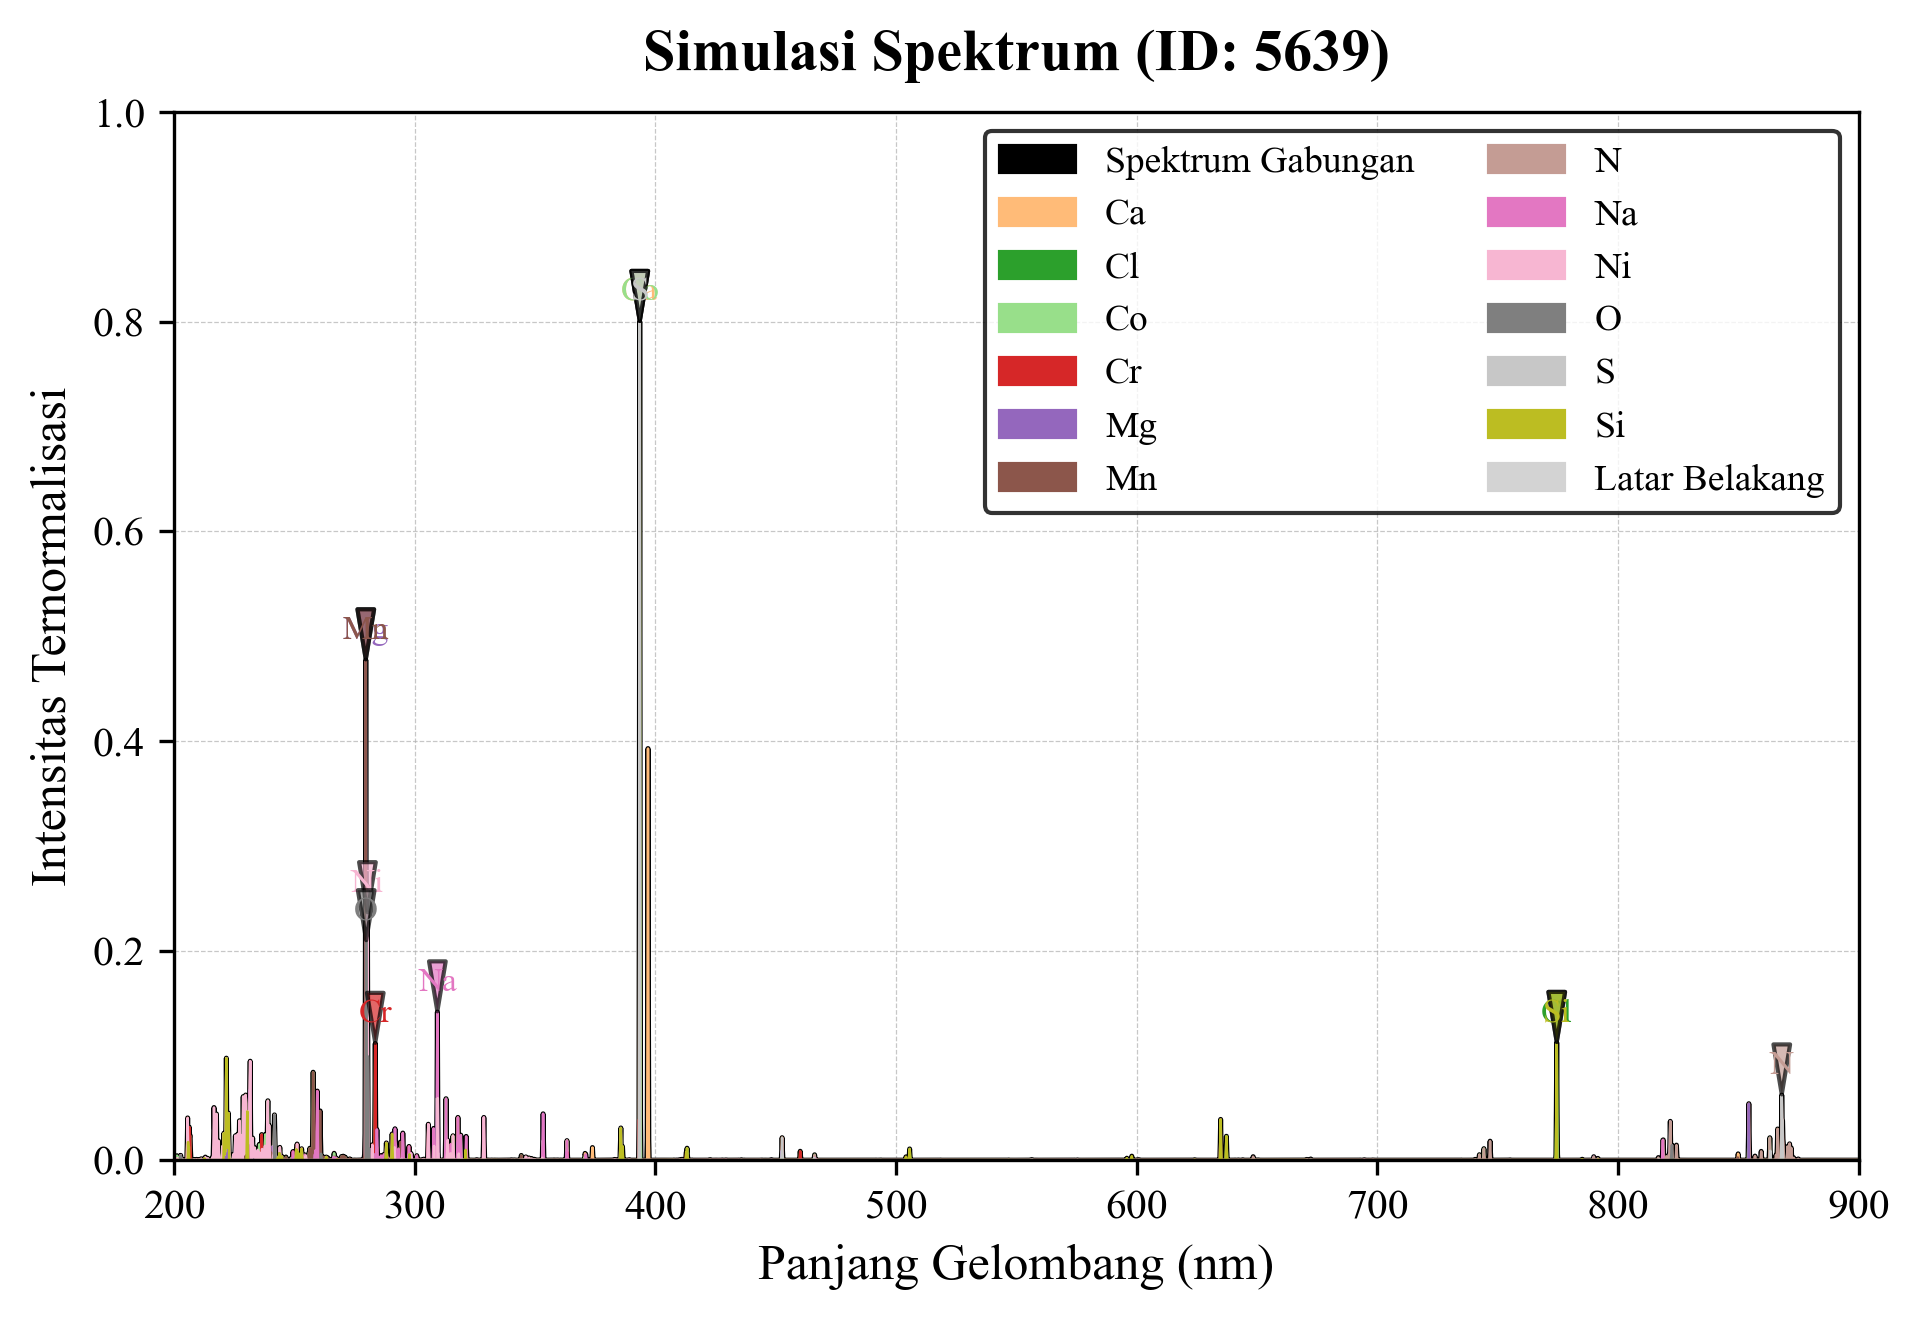
\includegraphics[width=0.9\textwidth]{spectrum_5639.png}
    \caption{Spectral simulation plot for sample 5639.}
    \label{fig:spectrum_5639}
\end{figure}

\clearpage

\section{Sample: 2441}
\subsection{Simulation Parameters}
\begin{table}[h!]
    \centering
    \begin{tabular}{ll}
        \toprule
        \textbf{Parameter} & \textbf{Value} \\
        \midrule
        Temperature ($T$) & 9242 \,\si{K} \\
        Electron Density ($n_e$) & 1.87e+17 \,\si{cm^-3} \\
        \bottomrule
    \end{tabular}
    \caption{Simulation parameters for sample 2441.}
    \label{tab:params_2441}
\end{table}

\subsection{Composition Analysis}
\begin{table}[h!]
    \centering
    \begin{tabular}{lcc}
        \toprule
        \textbf{Element} & \textbf{Initial Composition (\%)} & \textbf{Actual Labeled Position (\%)} \\
        \midrule
        Al & 0.65 & 9.35 \\
        Ar & 5.52 & 17.70 \\
        C & 6.59 & 5.66 \\
        Ca & 8.22 & 3.66 \\
        Cl & 8.81 & 0.39 \\
        Co & 10.22 & 34.28 \\
        Cr & 2.34 & 9.69 \\
        Fe & 0.00 & 0.00 \\
        Mg & 9.61 & 8.54 \\
        Mn & 10.82 & 17.24 \\
        N & 0.84 & 9.67 \\
        Na & 1.53 & 8.06 \\
        Ni & 10.73 & 11.67 \\
        O & 7.75 & 4.15 \\
        S & 5.03 & 3.71 \\
        Si & 4.22 & 5.32 \\
        Ti & 7.10 & 28.96 \\
        background & N/A & 19.02 \\

        \midrule
        \textbf{Total (\%)} & & 197.07 \\
        \bottomrule
    \end{tabular}
    \caption{Composition analysis for sample 2441.}
    \label{tab:comp_2441}
\end{table}

\subsection{Spectral Plot}
\begin{figure}[h!]
    \centering
    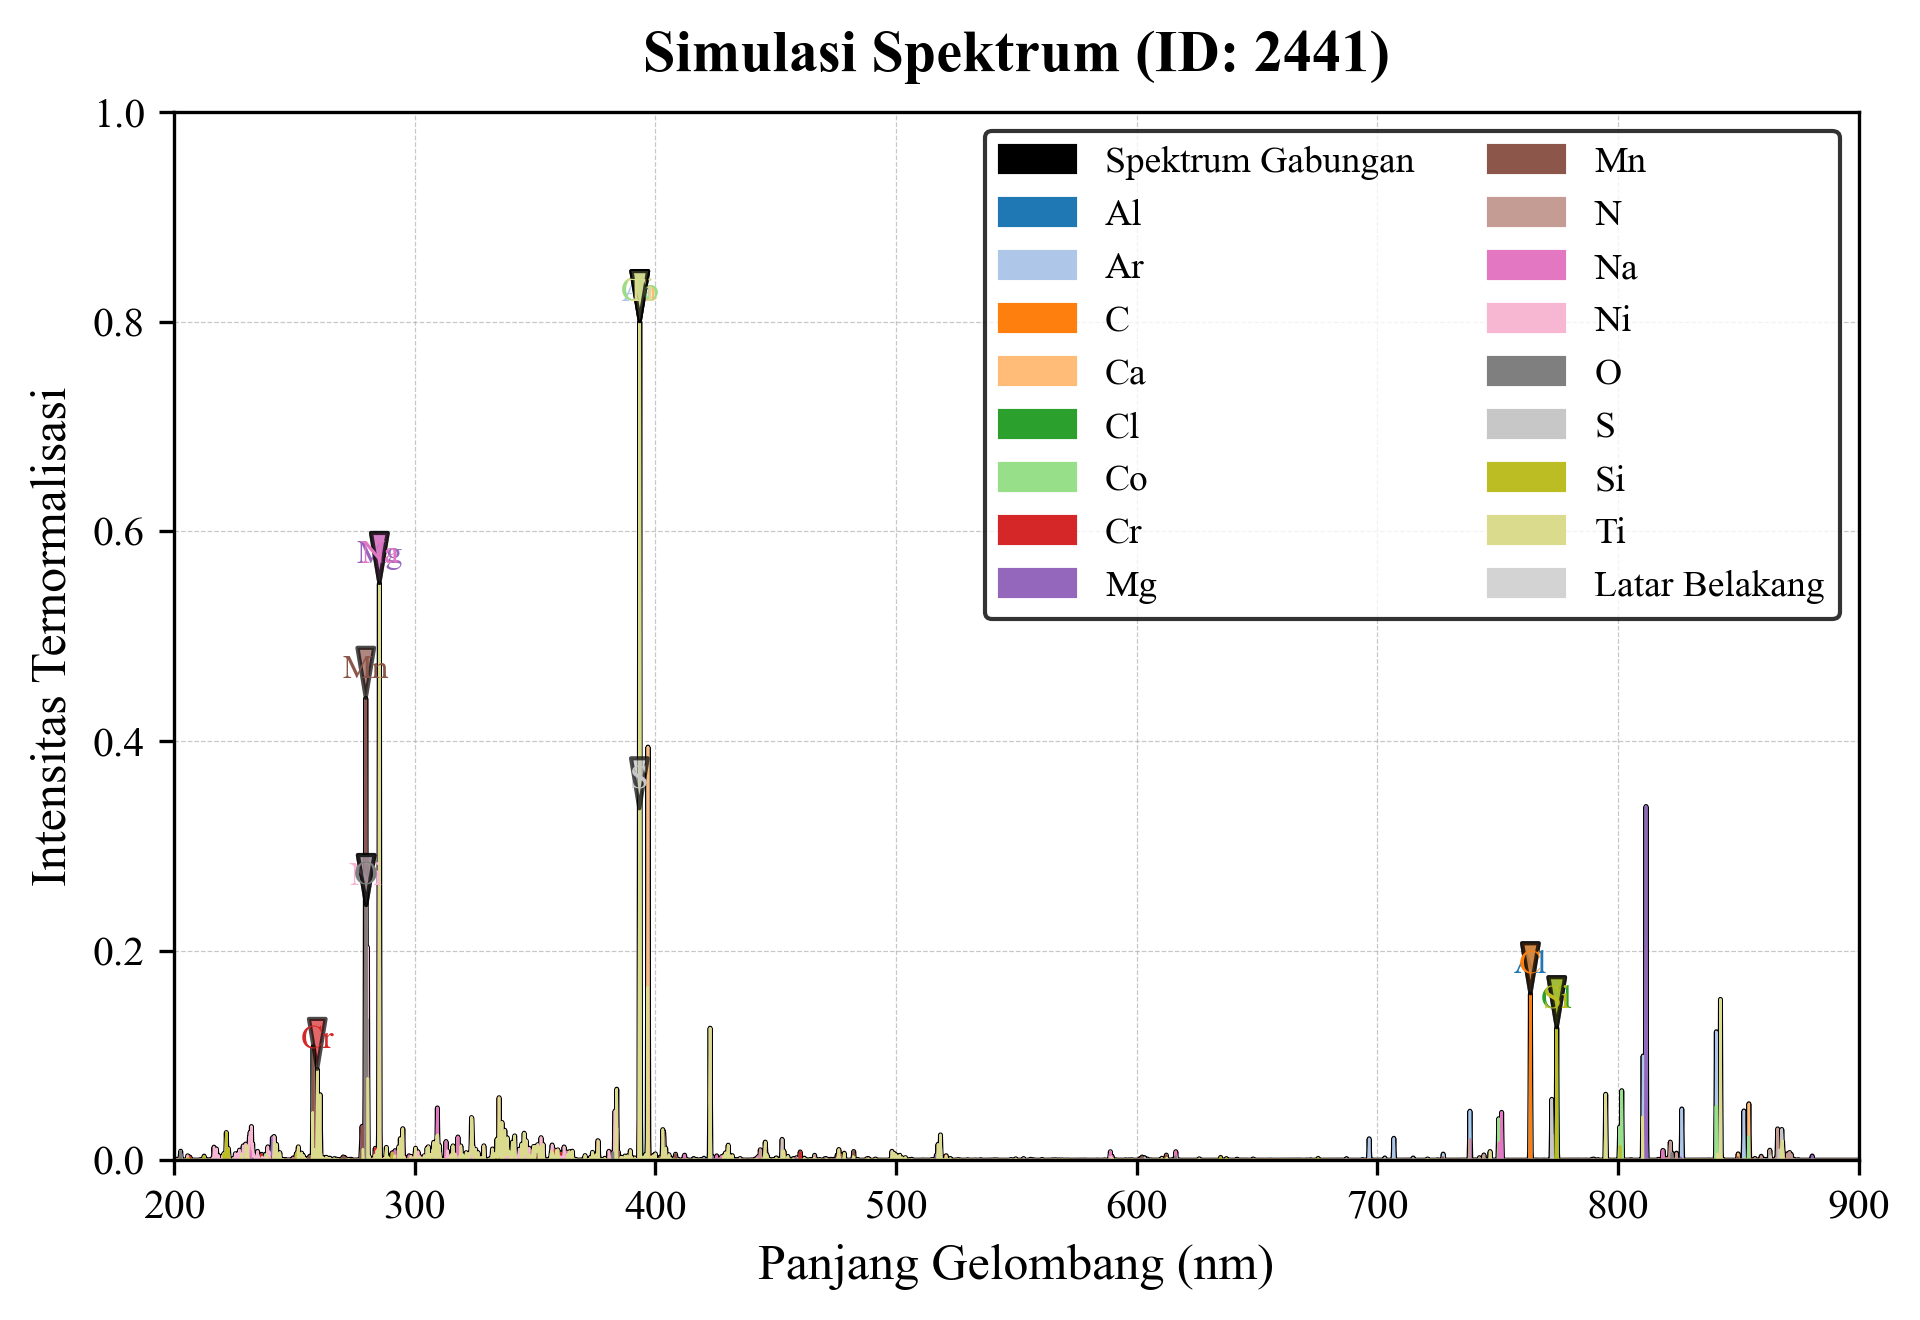
\includegraphics[width=0.9\textwidth]{spectrum_2441.png}
    \caption{Spectral simulation plot for sample 2441.}
    \label{fig:spectrum_2441}
\end{figure}

\clearpage

\section{Sample: 1644}
\subsection{Simulation Parameters}
\begin{table}[h!]
    \centering
    \begin{tabular}{ll}
        \toprule
        \textbf{Parameter} & \textbf{Value} \\
        \midrule
        Temperature ($T$) & 7424 \,\si{K} \\
        Electron Density ($n_e$) & 1.12e+15 \,\si{cm^-3} \\
        \bottomrule
    \end{tabular}
    \caption{Simulation parameters for sample 1644.}
    \label{tab:params_1644}
\end{table}

\subsection{Composition Analysis}
\begin{table}[h!]
    \centering
    \begin{tabular}{lcc}
        \toprule
        \textbf{Element} & \textbf{Initial Composition (\%)} & \textbf{Actual Labeled Position (\%)} \\
        \midrule
        Al & 2.66 & 5.32 \\
        Ar & 6.73 & 17.48 \\
        C & 2.49 & 5.40 \\
        Ca & 13.53 & 3.66 \\
        Cl & 0.84 & 0.29 \\
        Co & 0.00 & 0.00 \\
        Cr & 11.87 & 9.69 \\
        Fe & 0.00 & 0.00 \\
        Mg & 10.88 & 7.74 \\
        Mn & 12.83 & 17.24 \\
        N & 0.00 & 0.00 \\
        Na & 10.87 & 7.86 \\
        Ni & 6.46 & 11.67 \\
        O & 8.89 & 2.20 \\
        S & 0.84 & 0.61 \\
        Si & 5.56 & 5.32 \\
        Ti & 5.56 & 28.88 \\
        background & N/A & 33.28 \\

        \midrule
        \textbf{Total (\%)} & & 156.64 \\
        \bottomrule
    \end{tabular}
    \caption{Composition analysis for sample 1644.}
    \label{tab:comp_1644}
\end{table}

\subsection{Spectral Plot}
\begin{figure}[h!]
    \centering
    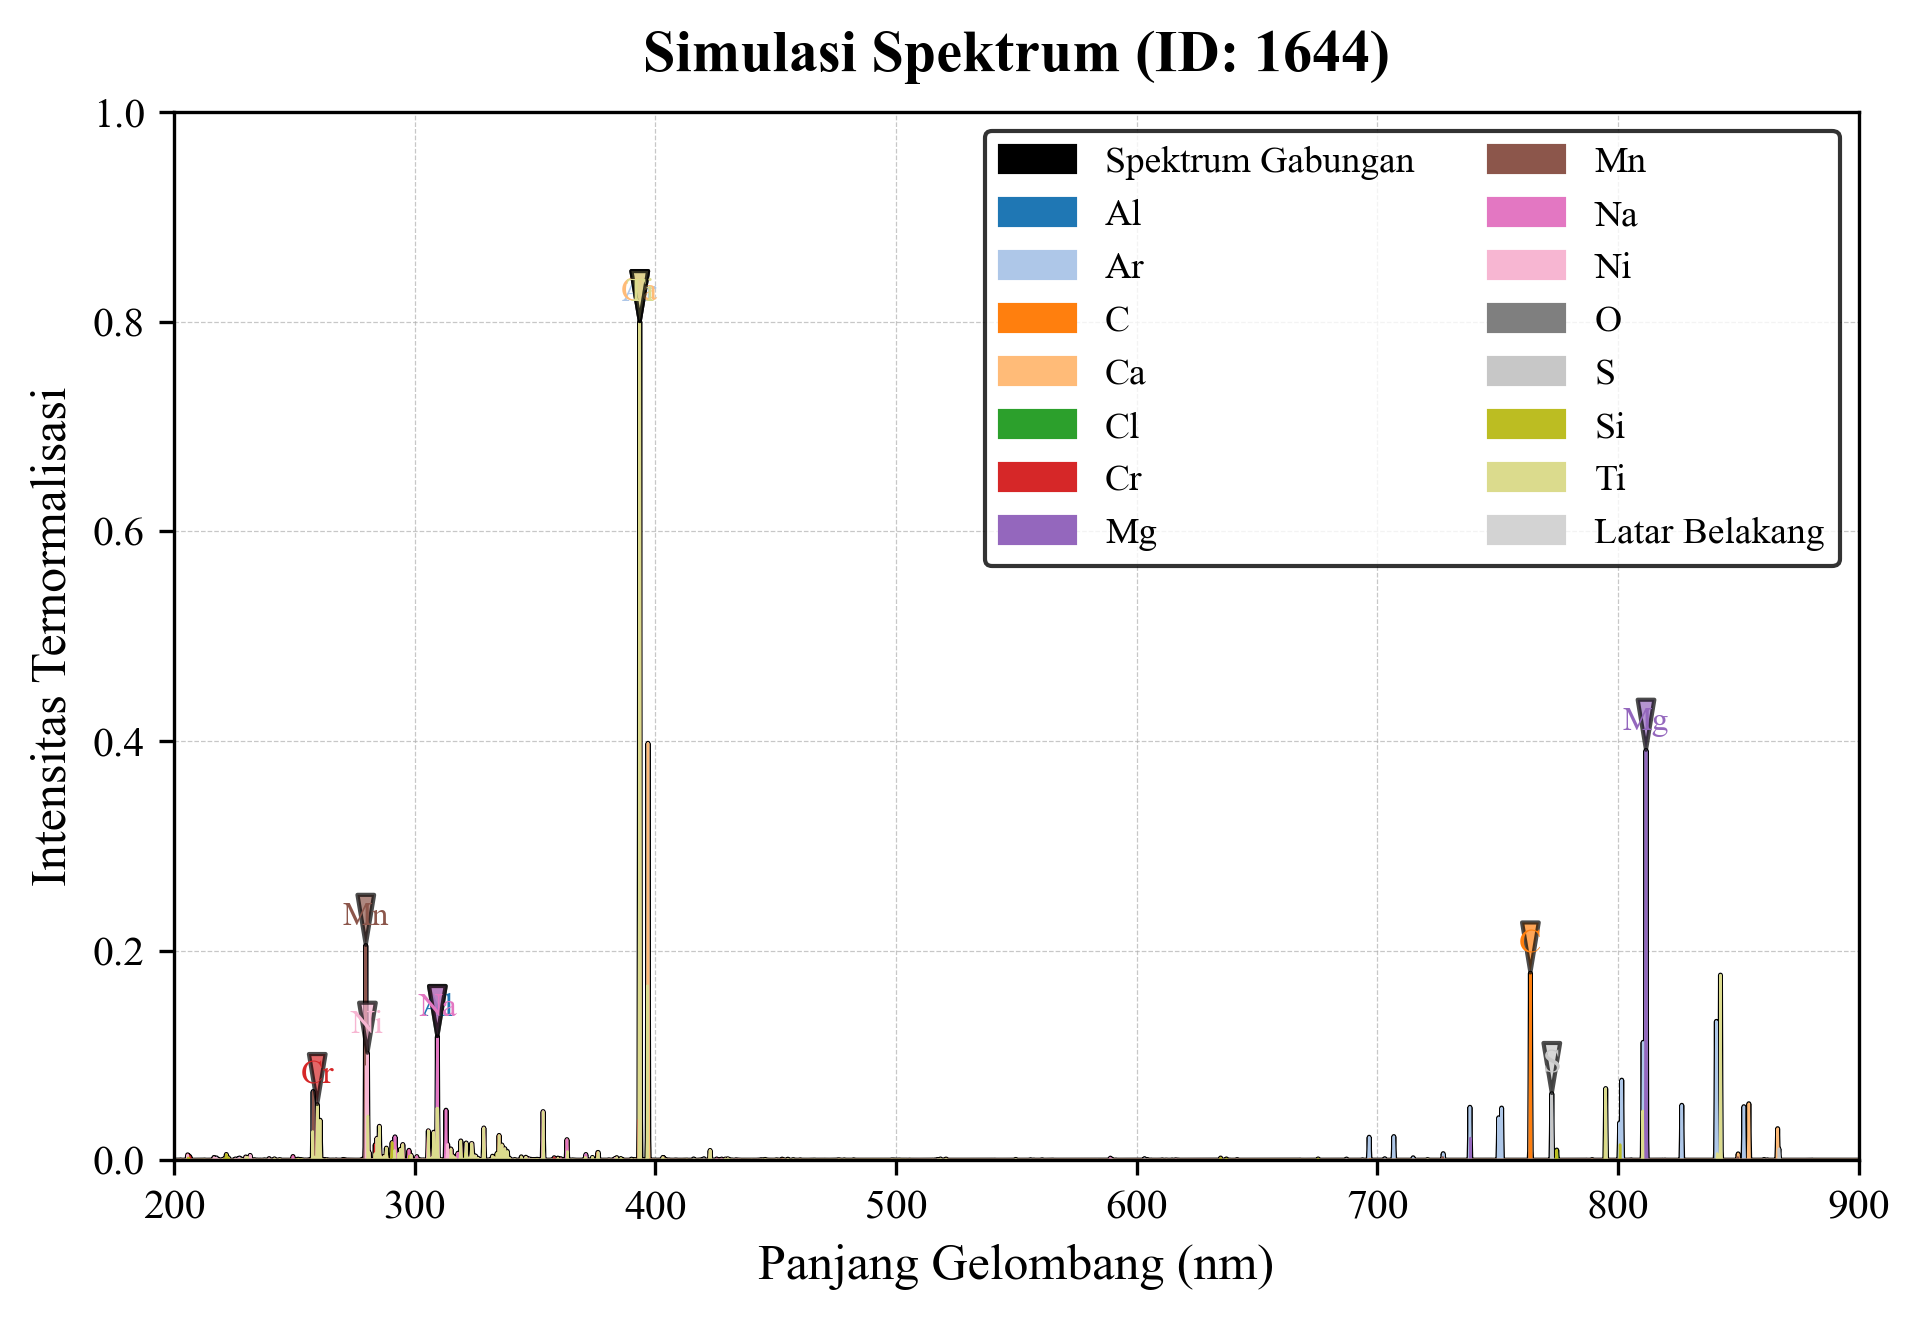
\includegraphics[width=0.9\textwidth]{spectrum_1644.png}
    \caption{Spectral simulation plot for sample 1644.}
    \label{fig:spectrum_1644}
\end{figure}

\clearpage

\section{Sample: 11151}
\subsection{Simulation Parameters}
\begin{table}[h!]
    \centering
    \begin{tabular}{ll}
        \toprule
        \textbf{Parameter} & \textbf{Value} \\
        \midrule
        Temperature ($T$) & 5707 \,\si{K} \\
        Electron Density ($n_e$) & 1.23e+15 \,\si{cm^-3} \\
        \bottomrule
    \end{tabular}
    \caption{Simulation parameters for sample 11151.}
    \label{tab:params_11151}
\end{table}

\subsection{Composition Analysis}
\begin{table}[h!]
    \centering
    \begin{tabular}{lcc}
        \toprule
        \textbf{Element} & \textbf{Initial Composition (\%)} & \textbf{Actual Labeled Position (\%)} \\
        \midrule
        Al & 6.92 & 3.32 \\
        Ar & 9.33 & 6.81 \\
        C & 6.83 & 2.88 \\
        Ca & 7.40 & 3.66 \\
        Cl & 10.20 & 0.29 \\
        Co & 6.52 & 20.70 \\
        Cr & 9.55 & 9.69 \\
        Fe & 3.55 & 52.08 \\
        Mg & 3.80 & 3.76 \\
        Mn & 8.12 & 15.50 \\
        N & 0.00 & 0.00 \\
        Na & 1.21 & 7.86 \\
        Ni & 4.07 & 11.67 \\
        O & 7.44 & 0.20 \\
        S & 10.94 & 0.61 \\
        Si & 2.25 & 3.81 \\
        Ti & 1.86 & 28.83 \\
        background & N/A & 26.66 \\

        \midrule
        \textbf{Total (\%)} & & 198.34 \\
        \bottomrule
    \end{tabular}
    \caption{Composition analysis for sample 11151.}
    \label{tab:comp_11151}
\end{table}

\subsection{Spectral Plot}
\begin{figure}[h!]
    \centering
    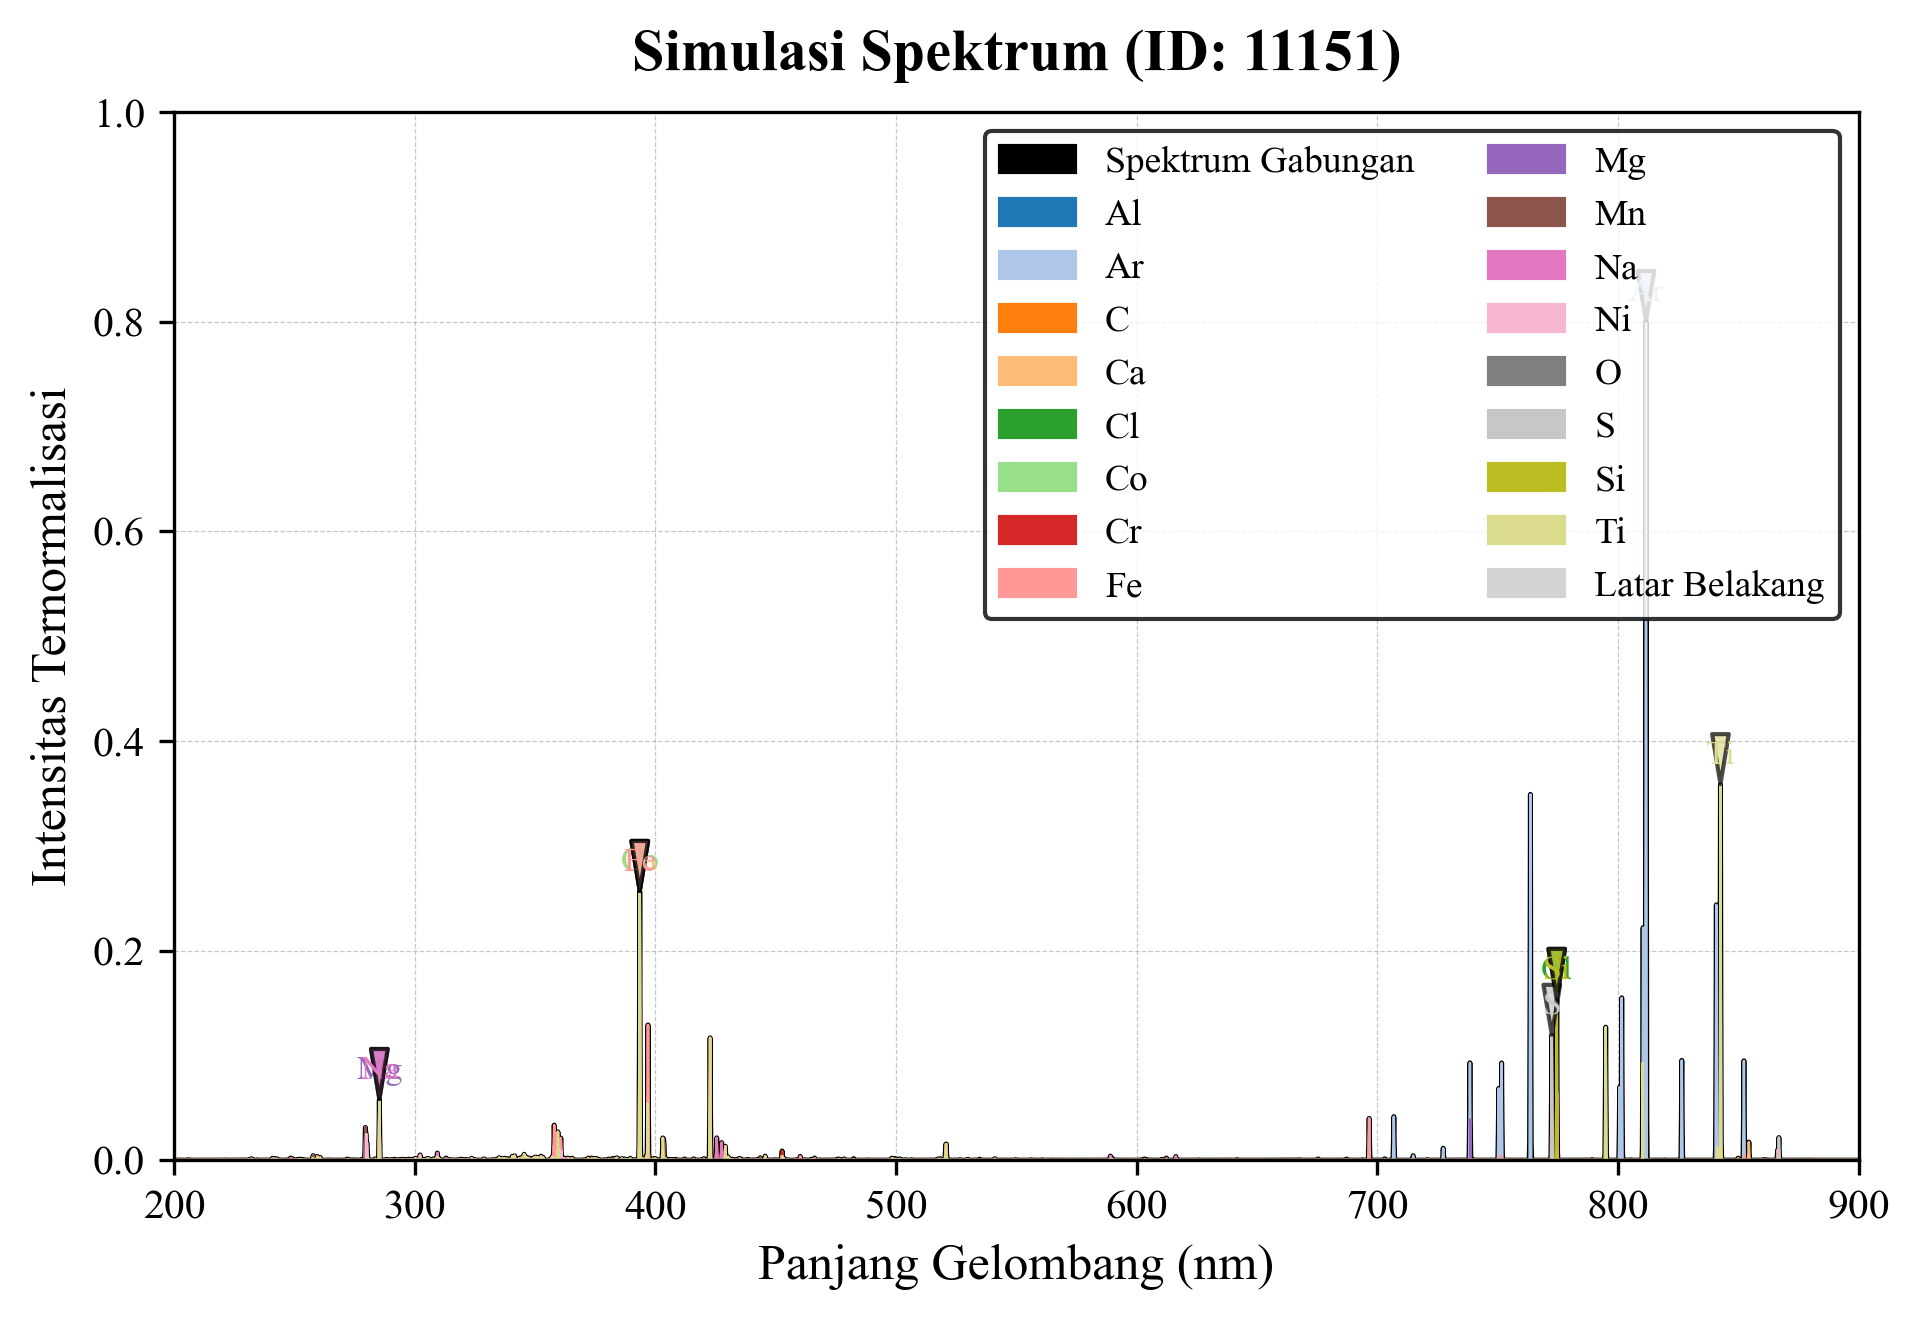
\includegraphics[width=0.9\textwidth]{spectrum_11151.png}
    \caption{Spectral simulation plot for sample 11151.}
    \label{fig:spectrum_11151}
\end{figure}

\clearpage

\end{document}
